\documentclass{article}
\usepackage[utf8]{inputenc}
\usepackage{amsmath}
\usepackage{amssymb}
\usepackage{color}

% For figures
\usepackage{graphicx} % more modern
%\usepackage{epsfig} % less modern
\usepackage{subfigure} 

\newtheorem{definition}{Definition}

%\newcommand{\comment}[3]{}  % suppress comments
\newcommand{\comment}[3]{{\color{#1} {\bf #2 :} #3}}

\newcommand{\yoav}[1]{\comment{magenta}{Yoav}{#1}}
\newcommand{\piya}[1]{\comment{blue}{Piya}{#1}}
\newcommand{\peter}[1]{\comment{purple}{Peter}{#1}}
\newcommand{\rayan}[1]{\comment{red}{Rayan}{#1}}
\newcommand{\alex}[1]{\comment{green}{Alex}{#1}}

%math symbols
\newcommand{\R}{\mathbb{R}}
\newcommand{\rad}{\mathcal{R}}
\newcommand{\sign}{\mathrm{sign}}


\title{HDR TRIPODS: From detection to reaction - computation in resource constrained sensor networks}
%\author{yfreund }
\date{March 2019}

\begin{document}

\maketitle

\section{Summary}
Any agent, be it a human, an animal or a robot, has to react to it's environment to take advantage of opportunities and to avoid dangers. The transformation of events to reaction can be partitioned into three steps: {\bf(1)} {\bf physical events} are transformed by sensors into {\bf raw data}, {\bf (2)} Computation transforms the {\bf raw data} into a {\bf knowledge} (representation of the environment), and {\bf (3)} an {\bf action} is chosen based on the {\bf knowledge}.

The design of the sensors is dominated by considerations of sensitivity and resolution (temporal and spatial).  The goal is to detect the smallest, faintest and most transient signals,
by exploiting priors on the physical model of signal acquisition, and the geometry of signal representation. Computation is used to reduce raw data into an internal representation and then into actions. 

These days the leading architecture of reactive systems is wireless sensor networks. Sensor networks consist of large numbers of small independent units, each with sensors, computation and wireless communication. Such systems are constrained by power and communication bandwidth. 

One important consequence of these constraints is {\em pushing computation to the edge}. Instead of communicating the raw information from each sensor to a central computer, each sensor unit locally computes summaries, or sketches, which are shorter and therefore cheaper to communicate. This also reduces the computation load on the units that receive the information.

\section{Framework}
\newcommand{\state}{\theta}
\newcommand{\estate}{\hat{\theta}}
\newcommand{\signal}{x}
\newcommand{\dtime}{t}
\newcommand{\ctime}{\tau}

This proposal combined several related lines of work. To facilitate the exposition, we start by introducing some terminology and notation that will be used throughout.

\begin{figure}[t]
\centering
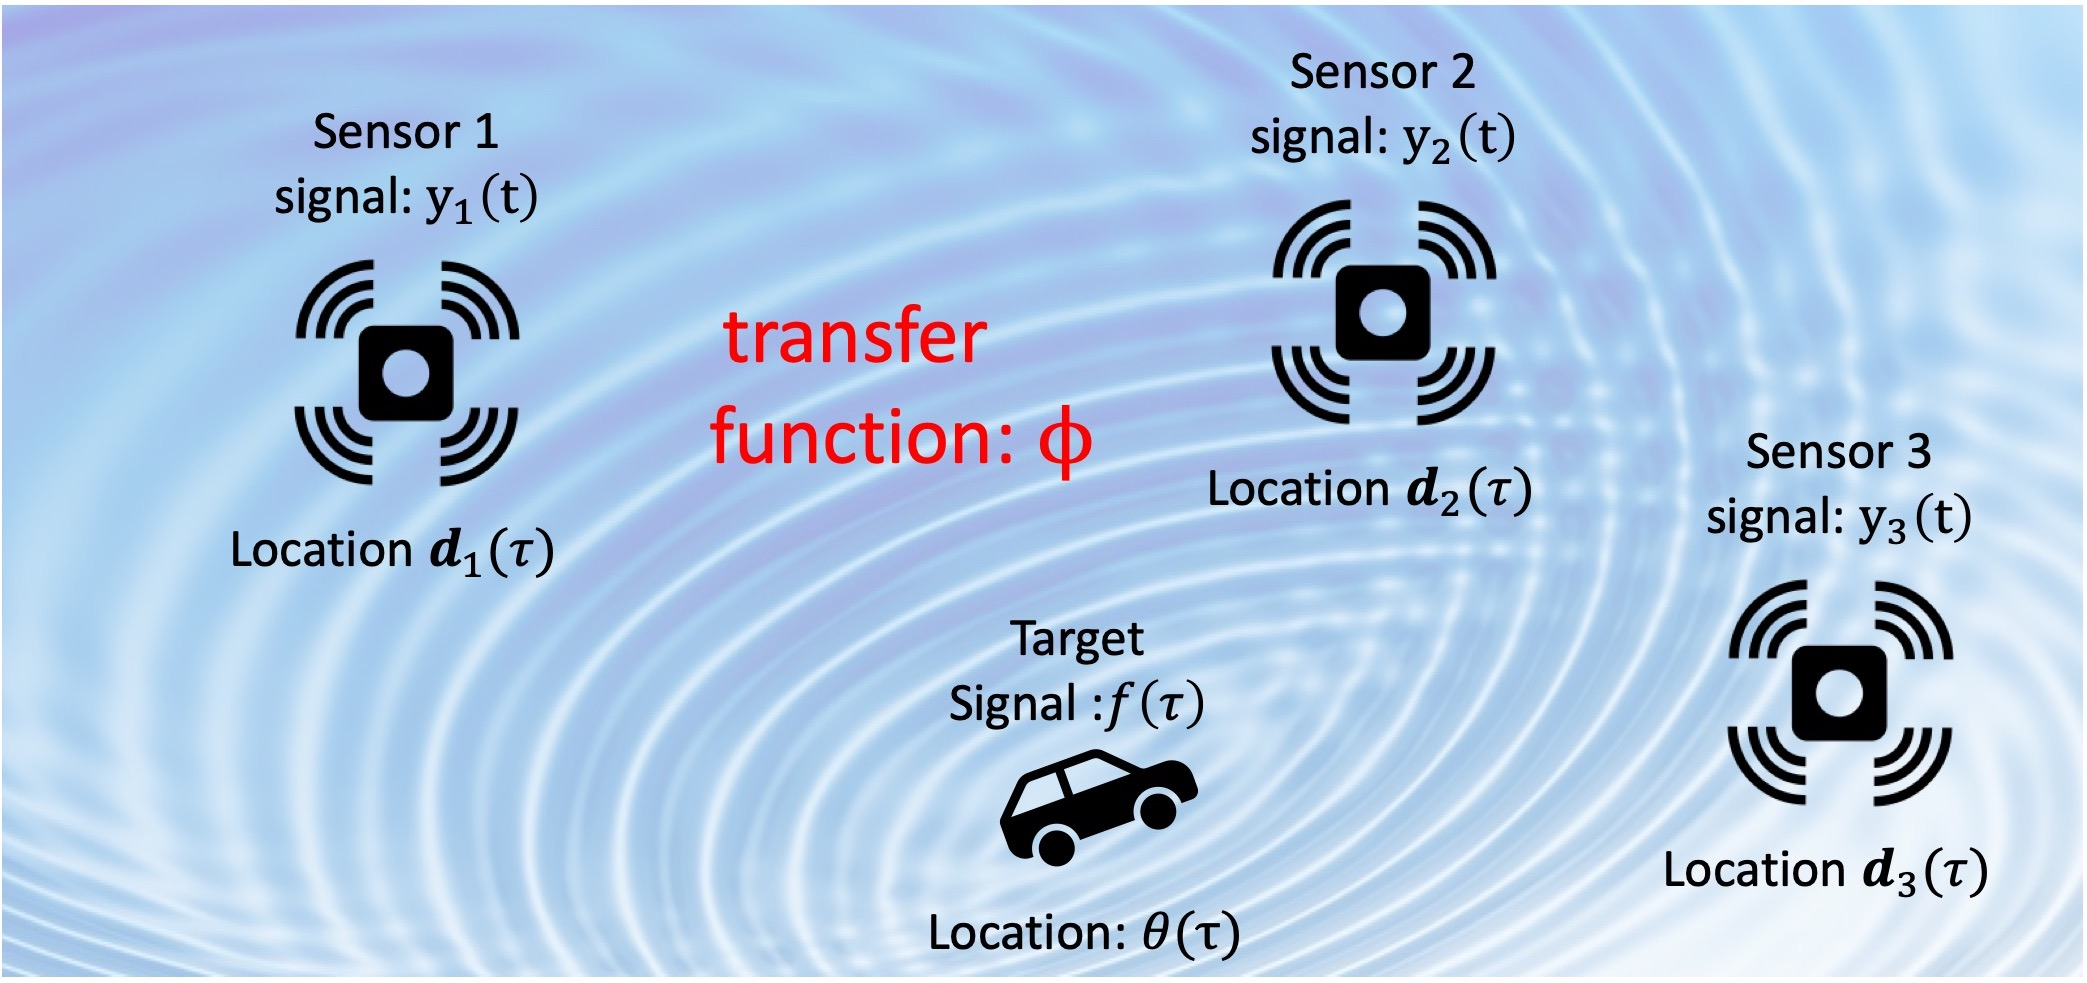
\includegraphics[width=0.9\columnwidth]{figs/Framework.jpg}
\caption{A schematic of a prototypical sensor network and associated
  notation\label{fig:prototypicalSensorNetwork}}
\end{figure}

We assume the sensor network is monitoring a physical system or space which is changing over time. We denote the {\em state} of the physical system at time $\ctime$ by $\state(\ctime)$ where $\ctime$ is continuous time. The nature of $\state$ will depend on the particular system. When tracking the location of a moving object the state would be a point in three dimensional space $\theta(\ctime) \in R^3$. When tracking the health of a bridge the state might be a function that maps locations on the bridge to the estimated stress and strain tensors for each location.

The task of the sensor network is to estimate the trajectory of the true state. We denote the estimated state by $\estate(\ctime)$. Our goal is to design a system that generates estimates $\theta(\ctime)$ that are close to the true states $\state(\tau)$. The quantification of this approximation will depend on the application.

Each sensor produces a sequence of measurements, which we call the {\em signal}. As we are focused on digital systems, we assume that the signal is a sequence of binary encoded numbers. We use $\dtime =1,2,3,\cdots$ to denote the discrete time used in each sensor. We denote a signal by $\signal_1,\signal_2,\cdots$.

%\yoav{In reality, sensor clocks are not synchronized and communication has non-zero latency. While this is the case, I think it is better to ignore this issue in this proposal.}

The relation between the state $\state$ and the signal depends on properties of the physical environment as well as properties of the sensor. The result is that often the signal from one sensor is insufficient to produce a good estimate $\estate$. By carefully combining the signals from several sensors, it is possible to generate a good estimate.

We denote the signals generated by sensor $i$ at time $\ctime$ as $\signal_i(\ctime)$. We assume that each sensor is equipped with a computer and with a communication channel. The focus of our work is on algorithms that transform signal sequences to other sequences and send/receive such sequences. The final product of this communication and computation is one or more estimates $\estate(\ctime)$.

%\yoav{Once again, I am ignoring the difference between $\ctime$ and $\dtime$. We should probably say something about it, Piya?}

\iffalse
For example, the signal captured by a microphone located a few feet away from a speaker in a reverberating room will record a highly distorted signal. The distortion is a result of echoes, reverberation at resonance frequencies, as well as noise and sounds from other sources. This signal is typically not very useful for either reproduction (
\fi
\subsection{Examples}
\begin{enumerate}
    \item {\bf Localization:} Peter's work using seismic sensor network to detect cars and train using Graph Signal processing\cite{riahi2017}. The "Sloocalization" paper on localizing passive RFID tags by integrating over a very long time.
    \item {\bf Anomaly detection} using a network of cameras and or microphones for low communication and low energy detection of anomalous events. Examples: cameras monitoring a highway. Microphone on factory floors. Smart-homes for the elderly living alone. Building security.
    
    An interesting part here is creating a model for what is normal with little or now intervention. Can we create a sketch of the signal which would be useful for defining the "normal" and distinguishing it from the abnormal?
\end{enumerate}

\iffalse
\section{Prompts}
These prompts are intended as starting points for sections in the proposal description. The names attached are my wild guess as to whom might interest.

\begin{itemize}
    \item (Piya): Optimizing sensor locations in space. (Rayan/Piya?): Possibly related problem: Unknown (or imperfectly known) sensor locations. {\peter That is array calibration and has been studied much in SP}
    \item (Piya): Suppose we use a sensor array to localize a target. What is the minimal amount of communication between sensors that is needed in order to achieve localization?
    \item (Peter) What are the theoretically minimal resources to perform analysis of seismology / noise. {\bf Peter} I dont think my research focus will be seismology in this proposal. if needed, can do it for proposal. {\bf Yoav} Peter, can you describe some theoretical problems that are interesting for you?
    \item {\peter Focus on the spatio-temporal fields in a  sensor network}
    \item (Rayan, Yoav, Alex): Statistical analysis on sketches. Sub-problems: Anomaly detection. Distribution drift. Creating long-term statistical models (Cars on highway, Factory floor, foot-traffic, engine monitoring){\peter seems interesting}
    \item (Rayan) Learning fast transforms (to reduce computation cost at sensors) 
\end{itemize}
\fi

\section{Difference based communication}
We propose a general framework for designing and analyzing sensor networks. Suppose we have two sensors two sensors whose task is to track state of target whose trajectory is defined by $\state(t)$. Suppose the sensors use a dynamic model to predict future states. For the sake of concreteness, suppose a Newtonian model of motion is used which predicts constant velocity of the target unless a disruptive force acts on it.

Let $\estate_1(t),\estate_2(t)$ be the estimates of the target location for each sensor. {\em In addition, each sensor maintains an estimate of the estimate of the other sensor.} $\estate_{1,2}(t),\estate_{2,1}$. Each sensor updates it's estimate of the velocity of the location of the target according to the signal it measures, but it does not update it's estimate of the other's estimate.  If the two estimate are close to each other $\estate_i(t) \approx \estate_{i,j}(t)$ then sensor $i$ sends no information to sensor $j$. On the other hand, if $\estate_i(t)$ is far from $\estate_{i,j}(t)$, then $\estate_{i}$ is transmitted from sensor 
$i$ to sensor $j$. Thus if the target is moving in constant speed, uninterrupted, there is not communication between the sensors.

The basic idea here is that a sensor sends out information only if
that information cannot be predicted by the receiver. Similar ideas
have been used in arithmetic coding and \yoav{I think} in
$\Sigma\Delta$ encoding.

Recently, PI Freund~\cite{TMSN} proposed an asynchronous computation
model called ``Tell Me Something New'' in which each agent broadcasts
a message only when the estimate it computes differs from the existing
estimates in a statistically significant way.

 One important application of sensor networks is to monitor activity
 and identify anomalies. Examples include: building security systems,
 factory floors, highway monitoring, health monitoring for the sick or
 elderly and many others.

 On its face, this might seem like an under-constrained impossible
 problem. However, note that for all of the environments listed above
 there is a highly repetitive pattern from day to day and from week to
 week. Add to that the sensors are stationary, and one would expect
 that most sensors observe highly regular and highly predictable
 patterns.
 
 The approach we propose in this case is that each sensor creates a
 model of the characteristics of the signals that it observes during
 normal operations. It alerts neighboring sensors if it observes
 something that is abnormal, i.e. a signal that has very low
 probability according to the model. When several sensors send an
 alert with a short time window, and when the alerts are consistent
 with each other, a global alert is sent to the human operators.

\section{Distributed signal processing}

Consider a source of a time signal, it can be a source of sound or vibration, it can be an electromagnetic signal such as WiFi. In the simplest version we consider a stationary point source that is emitting a signal in continuous time: $f(t)$

A stationary sensor network is measuring the signal as transformed by the environment transfer function. The network, as a whole, has one of a set of goals listed below

\begin{itemize}
    \item Recovering the transfer function of the environment in order to estimate properties of the environment. As, for example, Sonar or Seismology. This typically requires that $f(t)$ is under our control.
    %\item Reconstructing the original signal $f(t)$.
    \item Estimating the location of the source, especially if the source is not stationary.
    \item In the case of many sensors, selecting a subset of the sensors that is sufficient for the task.
\end{itemize}

Good algorithms for reaching these goals exist in the centralized computation setting. In other word, if we assume that all data is  transmitted to a single computer and processed together. We seek solutions for the setting where the communication bandwidth between sensors is restricted.

Some interesting extensions of the basic model. More than a single source exists (the cocktail party problem) or the source is not a point. The sources or the sensors are not stationary. 

As the source locations are in three dimensions of physical space, can we learn the 3D manifold of the signal properties? (cite)


\piya{\em [From source localization perspective, it will be good to mention two or three different types of models. For example, a network of distributed radars (for example, on smart cars) should be modeled differently from a network of cameras.) Maybe Peter can also suggest some realistic models. For now, I am using a somewhat generic model.]}

\rayan{\em [Not sure this is the right place for this comment, but here goes: One interesting class of problems that we can consider are "blind" or semi-blind problems, e.g., radar placed on ships where the exact locations of the ships is not known. There is some recent work from industry on problems of this type but with almost no theory whatsoever.]}

\subsection{Model for Localization (Piya)} A sensor network consisting of $M$ sensing units aims to capture information of interest (often described in terms of parameters) regarding the physical environment by acquiring measurements in space (dictated by sensor locations) and in time (dictated by the sampling technique employed at each sensor). In many applications (especially those concerning high-resolution/super-resolution imaging), the goal is to detect certain parameters $\theta_i\in\mathbb{C}^P, i=1,\ldots,K$ from $K$ targets of interest in the environment by acquiring signals emitted by them. 

\yoav{This describes a more general framework, using $\mathbb{C}^P$ (does that mean each coordinate is complex?). What is gained from this generality? maybe drop the general notation? Also how does high resolution/super-resolution fit here? If you have worked on such problem, I suggest you devote a paragraph and cite, rather than just mentioning in passing.} 

As an example, consider a network consisting of active radar units (for example, those mounted on autonomous vehicles) attempting to create a map of the environment. In this case, $K$ can denote the total number of pedestrians, bicyclist's and other cars and $\theta_i\in\mathbb{R}^3$ for the $i$th target will consist of its location $\mathbf{x}_i=[x_i,y_i]^T$ and velocity $(v_i)$ parameters, i.e.
\begin{equation} \theta_i = [ x_i, y_i, vx_i ,vy_i]^T, \quad 1\leq i\leq K  
\end{equation} 
\yoav{Shouldn't $K$ be estimated?}
%\rayan{It could also be 3 dimensional :), as can position}
Mathematically the space-time measurements collected at the $m$th sensing element can be described as \begin{equation} 
y_m (t) = \sum_{i=1}^{K} \phi (\mathbf{d}_m,\theta_i,t) + w_m(t), \quad 1\leq m\leq M
\end{equation}
where $w_m(t)$ is the additive noise. Here $\mathbf{d}_m\in \mathbb{R}^3$ denotes the location of the $m$th sensor and the function $\phi(.)$ characterizes the measurement model (often referred to as the point-spread function in the context of imaging) that depends on the physical laws governing wave propagation, and properties of the medium. Depending on the application and model assumptions, the function $\phi(.)$ can be linear, non-linear, and potentially, even non-convex. However, it can be {\em partially designed} by choice of senor locations $\mathbf{d}_m$. This will be a key enabler towards obtaining compressed sketches of measurements (or reducing the number of sensing units) while preserving the ability to reliably infer the parameter $\theta_i, 1\leq i\leq K$.\\
\yoav{We should define, in the introduction, some repeating terms, including compressed sensing and sketches. Maybe also more technical terms such as kernel, low rank matrices and low magnitude vectors/matrices.}

The basic model assumes targets as point sources, but in many situations, they are distributed. \piya{Perhaps Peter can help characterize this model, since SONAR deals with such targets}. 

\subsection{Central Objective and Role of Sensing Geometry (Piya)}
The main objective is to obtain estimates $\hat\theta_i, 1\leq i\leq K$ of the parameters of interest ($\theta_i$) using {\em minimal number of measurements/minimizing the number of sensing elements}. These estimates essentially are some appropriate functions of the spatio-temporal measurements $Y_T = \{y_m(t),  1\leq m\leq M, 1\leq t\leq T \}$, i.e., \begin{equation}
\hat{\theta_i}(T) = g_i (Y_T) 
\end{equation} 
In many scenarios, the parameters of interest can be reliably inferred from the {\em correlation of the measurements}. In other words, the correlation of the measurements act as a sufficient statistic for the parameters to be inferred. Depending on the application, the correlation matrix can be spatial (when the source signals are stationary), or spatio-temporal (when the temporal dynamics need to be tracked, such as for change-point detection). In these cases, we can effectively summarize the large amount of raw sensor measurements by only retaining and communicating their correlation. 
\yoav{The way I was thinking about it, each sensor has only one signal. In a one scenario, the quantity of interest is the "time delay of arrival" or the time shift of one signal relative to another that would maximize the correlation. Is there anything known about computing this time delay without communicating the whole time series?}

\noindent{\bf Spatial Correlation and Localization:} Suppose we compute the spatial correlation between $y_m(t)$ and $y_n(t)$  by averaging over $T$ time samples (the signals are assumed to be stationary over this interval) \footnote{Reasonable to do so when the source signals are stationary and emit independent signals. This is the common practice in source localization using antenna arrays. We can also use more sophisticated regularized estimation of correlation.}
\begin{equation}
r_{m,n} (T) = \frac{1}{T}\sum_{t=1}^{T} y_m (t) y^*_n (t) 
\end{equation} 
We can summarize the self and cross correlation between $M$ time-series measurements (collected at $M$ sensors) using these $M^2$ correlation values (collected in the form of a correlation matrix $R_T$). Owing to the geometry of the measurements, these correlation values directly depend on the sensor locations $\mathbf{d}_m$  (via the mapping $\phi(.)$). Hence, it is natural to ask 
\begin{enumerate}
\item Can we exploit the geometry of the measurement model to further compress the  correlation matrix $R_T$? What is the role of sensor geometry in this case? We should still be able reliably infer $\theta_i, i=1,2,\ldots, K$ from such a compressed sketch.
\item How large should $M$ be (in comparison to $K$) ?
\end{enumerate}

\section{Correlation-Aware Sensing (Piya)} 
With the aim of obtaining a compressive sketch of the correlation matrix (also termed as compressive covariance sensing), we will optimize the design of sensor array (i.e. choice of $\mathbf{d}_m, 1\leq m\leq M$) by understanding how the array geometry controls the algebraic structure of $R_T$. One of the main objectives will be to understand how much communication is needed (and between which subset of sensors) to achieve a certain level of accuracy. To illustrate this, we briefly discuss Co-PI Pal's recent work in structured sampler design (e.g., nested, coprime and generalized nested samplers) which utilize the idea of difference sets.

\begin{itemize}
\item {\bf Difference set-inspired Designs:} I will review some results in the context of array processing and DOA estimation...(to be filled in).
\item {\bf Proposed Research:} Motivated by these results, our goal will be to develop a rigorous framework for further developing the key idea of correlation-aware sensing to a distributed scenario and make it applicable for imaging problems beyond point target localization.
\begin{enumerate}
\item {\bf Distributed Sensing:} The idea of difference set inspired sampler design can be actually generalized beyond that of antenna arrays, to acquire {\em compressive sketches} of the correlation between signals acquired between pairs of sensors. In general, given $N$ sensors, it is natural to think that one needs to compute the correlation between all $N\choose 2$ time series (from all possible sensor-pairs) to construct the overall $N\times N$ correlation matrix $R_T$. However, using the idea of difference-set sampling, one can only compute  cross-correlation values between a much smaller subset of size $\Theta(\sqrt{N})$ of {\em suitably selected sensor-pairs} and recreate the entire $N\times N$ correlation matrix $R_T$. In the context of distributed sensing, this automatically means that only these sensors need to communicate and exchange information.

{\em Exploiting Distance-based Redundancies:} The key idea behind achieving such reduction is to exploit the redundancies present in the correlation values that naturally result from the physical spatial signal model. A widely used example of such a redundancy is that the correlation $r_{m,n} = E\Big(y_m(t)y^*_n(t)\Big)$ between $m$th and $n$th sensors is of the following form \begin{equation} r_{m,n} \approx f(\mathbf{d}_m - \mathbf{d_n}) \label{eqn:CorrRed}\end{equation}
In other words, the correlation is spatially only a function of the {\em inter-sensor distance}, and this is a direct consequence of the functional form of $\phi(.)$ \piya{Can give specific examples if needed}. This is also referred to as spatial stationarity and it is (exactly or approximately) true for many applications as narrowband and wideband radar \footnote{In the latter case, this holds at individual frequency bands after splitting the wideband signal into narrow frequency bins using a filter bank}, super-resolution optical imaging \cite{}, mmWave wireless channels \cite{} and so forth. Hence, depending on the inter-sensor distances, many of these $N\choose 2$ correlation values are actually repeated/redundant. Based on this observation, we propose to use a new sketching technique developed by co-PI Pal, called {\bf Generalized Nested Sampling (GNS) to reduce the amount of inter-sensor communication}. Suppose the sensors are located on a uniform grid. In one dimension, (\ref{eqn:CorrRed}) implies that the correlation matrix $R_T$ has Toeplitz structure and GNS provides an optimal way to select sensors to sketch such a matrix. 
\begin{definition}\piya{Definition of GNS goes here..}
\end{definition}
Hence, GNS dictates how to select a subset $\mathcal{S}_{\text{GNS}}$ of $M =  = \Theta(\sqrt{N})$ sensors out of $N$ available sensors. Let $R_{\mathcal{S}} \in \mathbb{C}^{M\times M}$ be the correlation matrix computed by aggregating the signals from these sensors. Then GNS ensures that $R_{\mathcal{S}}$ is a {\em lossless} sketch of the high-dimensional correlation matrix $R_T$. \piya{To Add (i) Finite sample performance guarantees (ii) two and three-dimensional extension (iii) low-rank extension and (iv) Time-varying model.}


%Will focus on what subsets of sensors in a distributed setting should communicate to be able to reconstruct the source scene. Can think of a subset of spatially close sensors to fully communicate with each other (assuming cost of communication proportional to proximity/distance), and then transmit the sketch / coarse parameter estimates (or their binarized measurement) to the sensors further away. Can lead to interesting hierarchical configurations for distributed sensors, dictated by $\phi(.)$. {\color{red} [To Add more Details..]}.
%\yoav{I think this is a very interesting question. Especially when the best subset depends on the location of the source.}\rayan{agree!}
\item {\em Beyond Point Target Localization: Using Priors and Sparsity} In many applications such as camera networks, the quantities of interest are not the low-level measurements acquired at the CCD sensors, but the processed images $I_t$. In such cases, we need to obtain a compressive sketch of the image $A (I_t)$ via the sketching operator $A (.)$ using low dimensional representation (over unions of subspaces or manifolds). In addition to conventional sparsity and low-rank priors, one can also utilize (partial) knowledge of the prior distribution of the images $I_t\sim~\mathcal{D}$. Utilizing these priors can lead to more effective compression for a given level of sparsity. {\color{red} [To be written..]}  
\end{enumerate}
{\color{red} These tasks can be further integrated with the binary embedding based sketching ideas proposed by Rayan and Alex.}
\end{itemize}

\section{Fast binary embeddings... (Saab, Cloninger,...)}
%\yoav{Please describe the algorithm (at least the outline)}

Often, distributed systems have severe bandwidth and energy constraints that necessitate extremely
coarse, e.g., binary, quantization of their measurements (e.g, \cite{fang2014sparse,boufounos20081}). Simple binary representations of data can be also quite appealing in hardware implementations, particularly if they are computationally inexpensive and consequently promote speed in hardware devices (\cite{jacques2013robust,le2005analog}). On the other hand, a major concern in using very coarsely sketched data is possible loss of accuracy when performing various tasks of interest, ranging from signal reconstruction to clustering and statistical hypothesis testing, among others.
\subsection{Background and Prior Work}Indeed a growing body of work, which co-PI Saab has contributed significantly to (e.g., \cite{SaabIEEEIT,knudson2016one,saab2018quantization,LybrandSaab2018,iwen2019new}), has focused on signal reconstruction from coarsely quantized compressive measurements. One important theme that emerges from this line of work  is that if one collects more coarsely quantized measurements than a critical minimal number, and uses sophisticated quantization schemes, then the extra measurements can be efficiently used in quantization-aware algorithms to rapidly drive the reconstruction error down.
%Recently the observation that sophisticated algorithms for coarse quantization when coupled with quantization-aware algorithms can exploit redundancy in the measurements to ob
Co-PI Saab has recently  extended this observation  beyond signal reconstruction, to the context of (Euclidean) distance-preserving binary embeddings \cite{huynh2018fast}. To be precise, we now briefly describe this contribution as it is pertinent to our ensuing discussion. In \cite{huynh2018fast}  $A: \R^n \to \R^m$ is a \emph{random} Johnson-Lindenstrauss (i.e., distance preserving) map and  $\mathcal{T}\subset \R^n$ is a set of finite or infinite cardinality. Moreover, $Q:\R^m \to \{\pm 1\}^m$ is a noise-shaping quantizer (e.g., a $\Sigma\Delta$ \cite{stuff} or $\beta$ \cite{stuff} quantizer). In their most commonly used form, noise-shaping quantizers act sequentially on the measurements, say $y_i$. For example, the simplest noise-shaping quantization scheme, the so-called greedy $1$st order $\Sigma\Delta$ scheme, is given, for $i=1,...,m$, by 
\begin{align}
    q_i &= \sign(y_i+u_{i-1})\\
    u_i &= u_{i-1} + y_i -q_i,
\end{align}
\yoav{How does one create an estimate of $y_i$ from $q_i$?}

where the state-variable sequence $u_i$ is initialized via, e.g., $u_0=0$. In matrix-vector notation, this yields the relationship $y=Du+q$  between the measurement vector, the state variables, and the resulting quantization, with $D$ being the $m\times m$ first-order difference matrix. Crucially both for the analysis and for practical implementation, this scheme is \emph{stable}, that is, $$\|y\|_\infty \leq c_1 \implies \|u\|_\infty \leq c_2,$$ for dimension independent constants $c_1,c_2$. More generally, other \emph{stable} noise-shaping quantizers act sequentially on the measurements $y_i$, %via carefully chosen functions $\rho,$
%\begin{align}
%q_i = \sign(\rho(y_i, u_i,u_{i-1},...,u_{i-r}))
%u_i = 
%\end{align}
%for carefully 
and yield relations of the form 
$$ y=Hu + q,$$ where $H$ is a lower-triangular matrix associated with the scheme. Quantizers of interest to us include
stable $r$th-order (with $r\geq 1$) $\Sigma\Delta$ schemes  \cite{}, with the relationship $y=D^r u+q$, and distributed-$\beta$ encoding schemes \cite{} where $H$ is a block diagonal matrix constituted of identical lower-triangular blocks, say $G$, given by $G_{i,i}=1, G_{i+1,i}=-\beta$, and $G_{i,j}=0$ otherwise.

With these quantization schemes playing a prominent role, in  \cite{huynh2018fast} co-PI Saab  constructed approximately isometric (i.e., distance preserving) embeddings between the metric space  $(\mathcal{T}, \|\cdot\|_2)$ and the binary  cube $\{-1,+1\}^m$ endowed with the pseudometric
$$d_{{V}}(\tilde{q},q) := \| {V}(\tilde{q} -{q}) \|_2$$
where $V$ is a carefully constructed matrix.
For a  matrix $A\in\R^{m\times n}$, and a noise-shaping quantizer $Q$, as above, the algorithm for computing these embeddings is simply given by \begin{align}
g: \mathcal{T} &\to \{\pm 1\}^m\nonumber\\
x &\mapsto q=Q(Ax).\nonumber
\end{align}
\rayan{Perhaps we need a section where we introduce background material like the  Johnson-Lindenstrauss lemma?}

In particular, when $A$ is a fast Johnson-Lindenstrauss matrix (e.g., \cite{}), the constructed embeddings support fast computation, and despite their highly quantized non-linear nature, they perform as well as linear Johnson-Lindenstrauss methods up to an additive error that decays exponentially (for $\beta$ quantizers) or polynomially (for $\Sigma\Delta$ quantizers)  in $m$. 
%\yoav{When exponentially and when polynomially?}
{Indeed, when $\mathcal{T}$ is finite} \cite{huynh2018fast} shows that with high probability %\RSnote{Careful: this should be $p$ not $m$ on the left}, 
and for prescribed distortion $\alpha$
\begin{align*} m \gtrsim \frac{\log{(|\mathcal{T}|)} \log^4 n}{\alpha^2} \quad \implies  \quad \big|d_{\widetilde{V}}(g(x), g(\tilde{x})) - \|x - \tilde{x}\|_2\big| & \leq {\alpha}\|x - \tilde{x}\|_2 + c\eta(m), \\ &\quad\text{where} \ \eta(m) \xrightarrow[m \rightarrow \infty]{} 0. \end{align*}
Above, $\eta(m)$ decays polynomially fast in $m$ (when $\mathcal{Q}$ is a $\Sigma\Delta$ quantizer), or exponentially fast (when $\mathcal{Q}$ is a distributed noise shaping quantizer). %In fact, we prove a more general version of the above result, which applies to infinite sets $\mathcal{T}$. 
%\medskip
{Additionally, when $\mathcal{T}$ is arbitrary (with possibly infinite cardinality, e.g., a compact manifold)} \cite{huynh2018fast} show that with high probability  and for prescribed distortion $\alpha$
\[ m \gtrsim \frac{\log^4 n}{\alpha^2}\cdot\frac{\omega(\mathcal{T})^2}{\rad(\mathcal{T})^2} \quad \implies \quad \big|d_{\widetilde{V}}(g(x), g(\tilde{x})) - \|x - \tilde{x}\|_2\big| \leq \max(\sqrt{\alpha},\alpha) \rad(\mathcal{T}) + c\eta(m)\]
where $\eta(m)$ is as before and where $\rad(\mathcal{T})$ and $\omega(\mathcal{T})$ denote  the Euclidean radius of  $\mathcal{T}$ and its Gaussian width (which roughly scales with the average radius of $\mathcal{T}$, so that intrinsically low-dimensional sets have a small Gaussian width). %, defined in Section \ref{sec:math_prelim}.
 In short, with \emph{very few measurements} compared to the ambient dimension of the signals, one can very efficiently (roughly at the cost of a fast Fourier transform) obtain low-dimensional binary sketches of the data. These sketches approximately preserve all pairwise distances in the original set and the distances in the embedded space can be computed efficiently.  
\rayan{may have to edit this depending on how the themes in the proposal evolve}

While signal reconstruction is not a major focus of our work, the promising results obtained in that context, and particularly in the context of binary embeddings, lead us to believe that the above techniques can be generalized to other tasks. 
%\yoav{I would differentiate between reconstruction, which corresponds to the lossy compression and compression methods whose output is designed to make particular types of inferences at the receiver end, rather than reconstruction. such as change detection, localization, statistical hypothesis testing. I think the former takes us into well trodden areas which have been studied in information theory, while the latter is much more of an open field. I recommend we focus on the latter.}
%\rayan{I agree. Reconstruction was intended as an example of a task that traditionally suffers from coarse quantization if care is not taken in designing the quantization algorithms, not as a focus of the proposal.}
Our goal  is to present a complete, theoretically rigorous, framework for performing various statistical, signal processing, and learning tasks from highly quantized data representations. We focus on the case of 1-bit representations as a theoretical extreme case, but emphasize that our methods should apply to more finely quantized data. We will propose, and analyze  (a) algorithms for  producing quantized sketches of data as well as (b) associated algorithms for performing the afore-mentioned tasks. Our strategy will be to develop these algorithms in tandem; that is, we will propose task-based quantization algorithms and quantization-aware algorithms for performing the tasks. We will strive for methods that support fast computation, and that lend themselves to distributed computing on, e.g., a sensor network.

\subsection{Models}
\newcommand{\transfer}{\phi}
  
Suppose signals of interest are modeled as $Y\in \mathcal{X} \subset
\mathbb{R}^d$, where $\mathcal{X}$ could be a finite set, i.e., a
point cloud, or an infinite set (e.g., a compact manifold, or the set
of all sparse vectors).
\yoav{In the discussion so far, the time $t$
  has a special role. Is $t$ one of the $d$ coordinates or is it an
  extra coordinate. In other words, should we use $Y(t)$ ?}

Alternatively, we may model signals as random vectors drawn according
to some distribution, i.e., $Y\sim~\mathcal{D}$ ofer $R^d$
\yoav{assuming that the signal for a single time point is generated by
  and IID draw from a fixed distribution seem unnatural in the context
  of a sensor network, where the state of the environment $\theta(t)$
  changes according to some dynamics.} where $\mathcal{D}$ accounts
for any structure in the signals. Further, assume that the measurement
operator, accounting for all the measurements at all the sensors, is
given by $\transfer:\mathbb{R}^d \to \mathbb{R}^m$, \yoav{I am
  assuming that $A$ is equal to the transfer function $\phi$ as described in
  the framework section and by Piya?}. In
the case of distributed sensing systems, we can assume each sensor
collects/computes a portion, $\transfer_i Y \in \mathbb{R}^{m_i}$, of
$\transfer Y \in \mathbb{R}^m$ (so that $\sum_i{m_i}=m$) and the corresponding portion
of ${Q}(Ax)$ where the quantization map $Q: \mathbb{R}^m \to \{\pm
1\}^m $ maps the measurements to bits. The sensors then must
collaborate to estimate a  quantity of interest,
such as the state of the target, 
$\theta(x)$ using and estimation function $f(Q(Ax)):=f\left(Q(A_1x),...,Q(A_kx)\right)\approx g(x)$.

\begin{equation}
x 
%\mapsto Ax = \left[ \begin{array}{c} A_1 x \\ \vdots \\ A_k x \end{array}\right] 
\mapsto Q(Ax) =\left[ \begin{array}{c} Q(A_1 x) \\ \vdots \\ Q(A_k x) \end{array}\right] \mapsto f(Q(Ax))\approx g(x)
\end{equation}


%\rayan{ Seems like in a model like this we could talk about Privacy (though I am not an expert on this -- any takers?} 


\subsection{Compressed Statistics}
\rayan{need a clear statement summarizing our goals here}
%\rayan{we need to unify the notation here. $g$ is being used differently than the previous section}
%\yoav{This sections needs more hand-holding of the reader. The way it is written assumed detailed prior knowledge. The more basic method - using unquantized kernels, needs some more explanation}.

The type of information that can be derived from $f(Q(Ax))$ depends on
the choice of measurement operator $A_i$ at each sensor, as well as
the quantization scheme.  For several of the tasks below, we will
design $f$, $A$, and $Q$ so that $\langle f(Q(Ax)), f(Q(Ay))\rangle$
approximates the Gaussian kernel $\langle g(x), g(y) \rangle =
e^{-\|x-y\|_2^2/\sigma^2}$.  As a first step, we will show that this
can be achieved by appropriately quantizing $cos(2\pi \langle w, \cdot
\rangle)$ for random choices of $w$ \cite{rahimi2008random}. To
achieve this in practice, each physical sensor could collect one or
more linear measurements $\langle \omega, \cdot \rangle$, and then the
(e.g., cosine) non-linearity could be implemented as part of the
quantizer. Alternatively, the sensor could measure the non-linear
function directly prior to quantization.

\subsubsection*{Background and Motivation}
\yoav{This section need to be re-written in a way that will make the
  connection to sensor networks clear. I don't know what are ``mean
  embeddings''. Can you describe them? I would focus on universal
  kernels unless there are good reason to talk about kernels that are
  not univrsal.}

There is a large body of literature around using a kernel $K:\mathbb{R}^d\times \mathbb{R}^d \rightarrow \mathbb{R}$ to define statistical distances through what's called \emph{mean embeddings} \cite{muandet2017kernel}.  A mean embedding $\mu_p:\mathbb{R}^d\rightarrow \mathcal{H}$ of a probability distribution $p$ is computed as
\begin{align*}
    \mu_p(z) := \mathbb{E}_{x\sim p} \big[K(z,x)\big].
\end{align*}
\yoav{what is $\mathcal{H}?$. It seems to me that if the kernel $K$
  maps into $R$ then $\mu_p$ should also map into $R$}


When $K$ is a \emph{universal} kernel (e.g. Gaussian, linear correlation) \cite{micchelli2006universal}, then the mean embedding satisfies a key property that $\|\mu_p - \mu_q\|_\mathcal{H}$ %(\rayan{define $\mathcal{H}$}) 
is bi-Lipschitz with respect to $\|p - q\|_{L^{\infty}}$ for absolutely continuous distributions $p$ and $q$.  This effectively means that the mean embedding transform maintains the same information as working in $\R^d$, with the benefit that mean embeddings also satisfy nice statistical convergence properties.  One key property is that, if we are only given $n$ finite samples $X\sim p$ and $Y\sim q$ to compute the empirical mean embeddings $\widehat{\mu}_X$ and $\widehat{\mu}_Y$, and we compute the mean embedding at all $z\in X\cup Y$, then $\|\widehat{\mu}_X - \widehat{\mu}_Y\|_2 \rightarrow \|\mu_p - \mu_q\|$ at a rate $O\left(\frac{1}{\sqrt{n}}\right)$.

However, statistics of this type suffer from a number of issues under computation and communication bottlenecks, as they requires storing and communicating all points in $X\cup Y$.
{\color{blue} In particular, computing $\hat{\mu}(z)$ at any one point $z$ requires evaluating the Kernel at all points in $X\cup Y$, which can be prohibitively expensive.}
This has motivated computational speed ups presented in \cite{cheng2017two} of undersampling $z\in S\subset X\cup Y$ under the condition that a kernel matrix $K$ can be decomposed as $K\approx RR^T$ for $R$ that can be efficiently accessed, as well as notions of kernel compression via randomized sketching \cite{gribonval2017compressive}.  However, even these approaches still require communication of a number of points between sensors, or passing double precision complex valued summary statistics.  

\subsubsection*{Goals}
Our overarching goal is to reduce the communication constraints by utilizing both sketching and binarization through use of $g(x) = f(Q(A(x)))$  {\color{blue} so that rather than communicate and compute with $x\in \R^d$ where $d$ may be large, one only needs to compute and communicate $(Q(Ax))\in \{\pm 1\}^m$, with $m\ll d$, or $f(Q(Ax))$}. In what follows, $\mathbb{E}_{x\in X} g(x)$ serves as a proxy for the empirical mean embedding of the data set $X$.  We aim to prove that this low complexity vector still converges to a type of mean embedding, and to provide a rigorous analysis of the statistical power, convergence rates, and minimal detectable separation criteria between the distributions.  Below we highlight the benefit of this approach in a number of different sensor problems.

\begin{itemize}
\item Two Sample Testing: 
%Assume the set of sensors collects a data set $\mathcal{X}\sim p_1$ for some distribution of points $p_1$, and a new data set $\mathcal{Y}\sim p_2$ for some distribution of points $p_2$.  An important question to ask is whether $p_1=p_2$, and whether this question can be addressed without communicating all data points from both sets. 
%\yoav{Do you mean "storing" or "communicating" the points. The second is what  seems more relevant here, but I don't understand what is communicated.}
%A modern approach to two sample testing, Kernel Maximum Mean Discrepancy \cite{Gretton 2012}, defines distances  between distributions by mapping each distribution to a Reproducing Kernel Hilbert Space through a smooth kernel $K$, and has existing results regarding consistency and power of the test.  However, construction of $K$ can be memory intensive, which motivated computational speed ups presented in \cite{Cheng, Cloninger, Coifman 2017} under the condition that a kernel matrix $K$ can be decomposed as $K\approx RR^T$ for $R$ that can be efficiently accessed.  Unfortunately these results cannot be efficiently implemented under power and communication bandwidth constraints, as they require passing individual data points between sensors.  
%Our goal is to eliminate these bottlenecks through the use of binarized embeddings like $g(x)$, which has the additional benefit of building a sketching of the data for appropriate choice of $A$.  
In the context of sensors, the two sample problem can be summarized as follows: a network of sensors collects the data set $X\sim p$ at some time (or location), and data set $Y\sim q$ at a later time (or different location), and the goal is to determine whether $X$ and $Y$ were distributed similarly.  To address this, we will analyze the binarized statistic $$\left\|\frac{1}{n}\sum_{x\in \mathcal{X}} g(x) - \frac{1}{m}\sum_{y\in \mathcal{Y}} g(y)\right\|,$$
%{\color{blue}Should we say this instead: we will construct functions $f$, so that $$\left\|\frac{1}{n}\sum_{x\in \mathcal{X}} f(Q(Ax)) - \frac{1}{m}\sum_{y\in \mathcal{Y}} f(Q(Ay))\right\|,$$}
%(\rayan{and its finite sample approximation?}), 
under appropriate norm, and seek to characterize the minimal conditions under which a deviation between $p$ and $q$ can be detected.   The approach requires characterizing the types of deviations $p - q$ that can be detected, namely those for which $$\left\|\int e^{-\|x-y\|^2/\sigma^2} (p(y) - p(y)) dy \right\| > \epsilon,$$ as well as the rates at which these deviations can be detected.
%a deviation of the type $\int K(x,y) (p_1(y) - p_2(y)) dy$ can be detected by $\mathbb{E} g(x)$\rayan{We probably need to clarify this sentence}.
The communication benefit of such a statistic is that the sensors need
only transmit the mean of $g(x)$, rather than all the individual
points.  Additional mathematical questions arise in the setting that
different sensors collect non-overlapping features from $X$, as this
creates a banded embedding matrix $A$.

\alex{Could expand on this, or reference other comments in proposal and a few papers about this for JL embeddings}
\yoav{I would like to see a more self-contained description, rather
  than an expansion. While I agree with the goals, I have no idea how
  the described math can be used to achieve those goals.}

%\yoav{Rather than describing the existing approach at the end, I would start with it and say, we plan to extend this approach ...}
%The approach builds on the existing literature of kernel Maximum Mean Discrepancy \cite{Gretton 2012} and the computational speed ups presented in \cite{Cheng, Cloninger, Coifman 2017} under the condition that a kernel matrix $K$ can be decomposed as $K\approx RR^T$ for $R$ that can be efficiently accessed. 
%One approach to two sample testing, Maximum Mean Discrepancy \cite{Gretton et al, 2012}, defines an unbiased distance between distributions as
%\begin{equation}
%    MMD(X,Y;\mathcal{F}) = \sup_{f\in \mathcal{F}} \left| \mathbb{E}_{x\in \mathcal{X}} f(x) - \mathbb{E}_{y\in \mathcal{Y}} f(y) \right|.
%\end{equation}
%As the number of samples $n\rightarrow \infty$, MMD is shown to detect any nonzero deviation $\|p-q\|_\infty$ when $\mathcal{F}$ is a Reproducing Kernel Hilbert Space \cite{Skolkoph}.  However, the method requires $\mathbb{O}(n^2)$ storage.
\rayan{let's refine this discussion a little -- I have some ideas here}

\item Change Point Detection: A variant of the two sample testing problem is change point detection, in which the data is streaming $X(t)$ according to some underlying stochastic process.  At some time $t^*$, the distribution of the stochastic process changes from one distribution to another, and the issue is how quickly after $t^*$ this change can be detected.   There exists a mean embedding approach to change point analysis \cite{Bach 2008} which uses the kernel Fisher discriminant ratio to measure the homogeneity between time segments of the process.  However, this once again requires storage of all points over the length of the detection window and communication of those points across sensors for both computing the window mean and variance. It also suffers from an inability to begin computing the change point statistic until all points in the window have been collected.  We aim to introduce the binarized sketching framework to produce an efficient computation to the kernel mean as in two sample testing, as well as a fast construction of a low rank approximation to the kernel covariance matrix.  We will derive it's new limiting distribution under the null model of no change, as well as the consistency under the alternative distribution when a change does occur.  

\item Multiple Sensor Common Factor Identification: A common issue is aggregating multiple sensors to identify and magnify the signal detected by both sensors.  Under a linear model, algorithms such as Canonical Correlation Analysis \cite{} act on multiple streams of simultaneously collected data $X_i(t)$ to filter noise and recover highly correlated linear projections from two the data sets.
Recently, a kernel CCA technique called alternating diffusion \cite{Talmon Lederman} has be used to identify common nonlinear effects by building a kernel $K_i$ from each sensing modality and analyzing the product kernel $(K_1 K_2)^t$.   Concretely, assume that there exists a hidden manifold $\mathcal{M}$ and two nuisance manifolds $\mathcal{N}_1$ and $\mathcal{N}_2$, and samples $s((x_i,y_i^{(1)}, y_i^{(2)}))$ for $(x_i,y_i^{(1)}, y_i^{(2)})\in \mathcal{M}\times \mathcal{N}_1\times \mathcal{N}_2$.  Due to sensor location or modality, sensor 1 collects data points $S_1 = s((x_i,y_i^{(1)}, \xi))$ and sensor 2 collecting data points $S_2 = s((x_i,\zeta,y_i^{(2)}))$.  Then roughly speaking, for some assumptions on $s$ and for $K_1: S_1\times S_1 \rightarrow \mathbb{R}$ and $K_2:S_2\times S_2 \rightarrow \mathbb{R}$, Talmon and Wu \cite{Talmon Wu} proved $(K_1 K_2)^t$ is the diffusion kernel on $\mathcal{M}$ only.   This is a very beneficial feature, as it means that one can compute kernel statistics for distributions defined on $\mathcal{M}$ only, independent of the nuisance features that may differ between sensors due only to modality or location.


However, this requires communication of all $n$ points across sensors to compute the kernel product.  We propose to analyze such approaches under minimal communication constraints by utilizing the low rank binarized decomposition $K_i \approx g_i(S_i) g_i(S_i)^*$.  As the key feature of alternating diffusion is computing the inner product matrix $g_1(S_1)^* g_2(S_2)$, which has dimension $d<n$ and is also low rank.  This implies it is possible to sketch $g_1(S_1)$ (resp. $g_2(S_2)$) with a small set of vectors $v_j$ (resp. $w_k$) and only communicate vectors $g_1(S_1)^* v_j$ (resp. $w_k^* g_2(S_2)$) such that $\mathbb{E}_{j,k}[g_1(S_1)^* v_j w_k^* g_2(S_2)] \approx g_1(S_1)^* g_2(S_2)$.  The amplification of the common factors observed by both sensors can serve to boost the power of the two sample and change point statistics on the shared observable manifold $\mathcal{M}$, as well as other compressed statistics that can be computed \cite{Griboval}.
%\yoav{This last item looks very interesting, but I don't understand it ... is it related to the problem I suggested of finding the offset of highest correlation for two similar signals?}
\end{itemize}

\section{Localization of weak sources (Peter)}

\yoav{Peter, I would like to see some discussion of using using sensor
  networks to estimate the transfer function, which, I think, is a
  main part of your past work.}

Detecting weak sources within a sensor network with or without a fusion center. The network could consist of sensors with know location, partially unknown or unknown positions.


\subsection{With a fusion center}
The propagation path from a given source location would here represent multiple propagation paths in a non-uniform media. The frequency domain transfer function from a source location to $N$ receivers ${\bf a}$. Assuming $K$ uncorrelated sources of complex amplitude $\bf s$ the received signal is 
\begin{equation}
{\bf y}={\bf A}{\bf s}+{\bf n},
\end{equation}
where ${\bf A}=[{\bf a}_1, \dots {\bf a}_k ]$  and $\bf n$ is uncorrelated noise. 
Forming the ensemble mean over multiple snapshots 
\begin{equation}
{\bf C}={\cal E}[{\bf y} {\bf y}^H]= {\bf A}{\bf s}{\bf s}^H{\bf A}^H+{\bf N},
\end{equation}
\yoav{What is ${\cal E}$?  What is the meaning of ${\bf y} {\bf y}^H$
  is it an inner or outer product? }

\subsection{Without a fusion center}
Here the processing is done locally at each node.

\subsection{Spatio-temporal fields}

\subsection{Use of a sensor network}
\begin{itemize}
\item Track an EM source in a home based on an ad hoc network. 
\item Estimating foot traffic (as in match point)
\item Localize a speaker in a room
\item Localizing a weak source in a floating network where the sensor locations are unknown. In e.g., The ocean
\item Structural monitoring using 
\item Localizing an acoustic source anywhere in a home using a sensor few sensors in a room. A human can do it. 
\end{itemize}



\section{results from previous grants}
%PETER: I commented it out as it is not important yet and was full of broken links.
% \subsection{Sampling and quantization theorems for modern data acquisition}
% %The investigator has not received prior NSF support.
% %\vspace{5pt}\noindent{\bf Results from Prior NSF Support:} 
% {Co-PI Saab: \em Sampling and quantization theorems for modern data acquisition (DMS-1517204, 08/01/2015--07/31/19,
% \$160,404)} 
% %   So far this grant has resulted in three journal articles \cite{KSW16, MS16, NSW16} and one journal submission \cite{SWY16}. \\
% %   {\bf Intellectual Merit:} Two of the above works \cite{KSW16, SWY16} pertain to the quantization of compressed sensing measurements. Specifically, \cite{KSW16} is the first result showing that \emph{scalar} 1-bit quantization allows the magnitude of sparse signals to be recovered from compressed sensing measurements, provided an affine shift is employed. \cite{SWY16} shows that a combination of Sigma-Delta quantization and an encoding step based on a discrete Johnson-Lindenstrauss embedding allows for a near-optimal rate-distortion relationship. The other two papers quantify how using prior information (in the form of a possibly erroneous support estimate) in conjunction with weighted $\ell_1$ minimization allows for improved recovery guarantees from fewer compressed sensing measurements when the support estimate is accurate enough. 
% % \\ {\bf Broader Impacts: }  In addition to dissemination of research results through seminars and workshop talks, Saab has developed and taught graduate courses on (1) compressed sensing and its applications and (2) applied and computational harmonic analysis. Additionally, he has mentored a (former) undergraduate (Steven Gagniere, currently at UCLA) in research on quantization of compressed sensing measurements (paper currently being written).   
% This grant resulted in 9 published or accepted journal articles \cite{KSW16, MS16, NSW16, SWY16, NSW17, LS2018, IPSV2018, HS2018, FKS17}, and 4 conference papers \cite{NSW17_conf, FKS17_conf, IPSV17_conf, ILNS19}.  {\bf Intellectual Merit:}  \cite{KSW16, SWY16, FKS17, LS2018, ILNS19} study quantization of compressed sensing (CS) measurements,  dealing with  $1$-bit scalar quantization, compression of  bit-streams,  circulant measurement matrices, and low-rank matrices, and manifold-valued signals. \cite{HS2018} develops a state-of-the-art technique, and accompanying theory, for embedding datasets into the binary cube while preserving Euclidean distances.  \cite{NSW17} provides a framework for using $1$-bit  measurements for classification  and analyzes the case of two clusters. The papers \cite{MS16, NSW16} show that using prior support information and weighted $\ell_1$ minimization yield improved recovery  from fewer CS measurements. Finally, \cite{IPSV2018, IPSV17_conf} study phase retrieval from local measurements. The works use and develop tools in random matrix theory, mathematical signal processing, and applied harmonic analysis.  
%   %Specifically, \cite{KSW16} is the first result showing that \emph{scalar} 1-bit quantization allows magnitude recovery from compressed sensing measurements, provided an affine shift is employed. \cite{SWY16} shows that Sigma-Delta quantization with an encoding step based on a discrete Johnson-Lindenstrauss embedding allows for a near-optimal rate-distortion relationship. \cite{FKS}The other two papers quantify how using prior information (in the form of a possibly erroneous support estimate) in conjunction with weighted $\ell_1$ minimization allows for improved recovery guarantees from fewer compressed sensing measurements when the support estimate is accurate enough. 
%  {\bf Broader Impacts: }  In addition to dissemination of results through multiple seminars and workshop talks, Saab has developed and taught graduate courses on (1) compressed sensing and its applications, (2) applied and computational harmonic analysis, and (3) mathematical methods in data science. He has  mentored a UCSD undergraduate (S. Gagniere, currently at UCLA) in research on quantization of CS measurements, and UCSD graduate students (E. Lybrand, A. Nelson, B. Preskitt, J. Liang), and postdocs (A. Ma, T. Huynh),  some of whom are co-authors on the works above, while others are taking part in ongoing work. Two of the above mentioned graduate students and postdocs are female, one is an air-force officer, and at least two are members of under-represented groups.%\hfill\\


\nocite{*}
\bibliography{tripods}{}
\bibliographystyle{unsrt}

\end{document}
